\section{Simulations}
\begin{equation}
    G(s) = \frac{K_s \cdot \Delta V}{1.159 s^2 + 5.365 s + 1}
\end{equation}

\begin{align}
    T_u  &= 0.1655 \\
    T_g  &= 5.9602
\end{align}

\begin{figure}
    \centering
    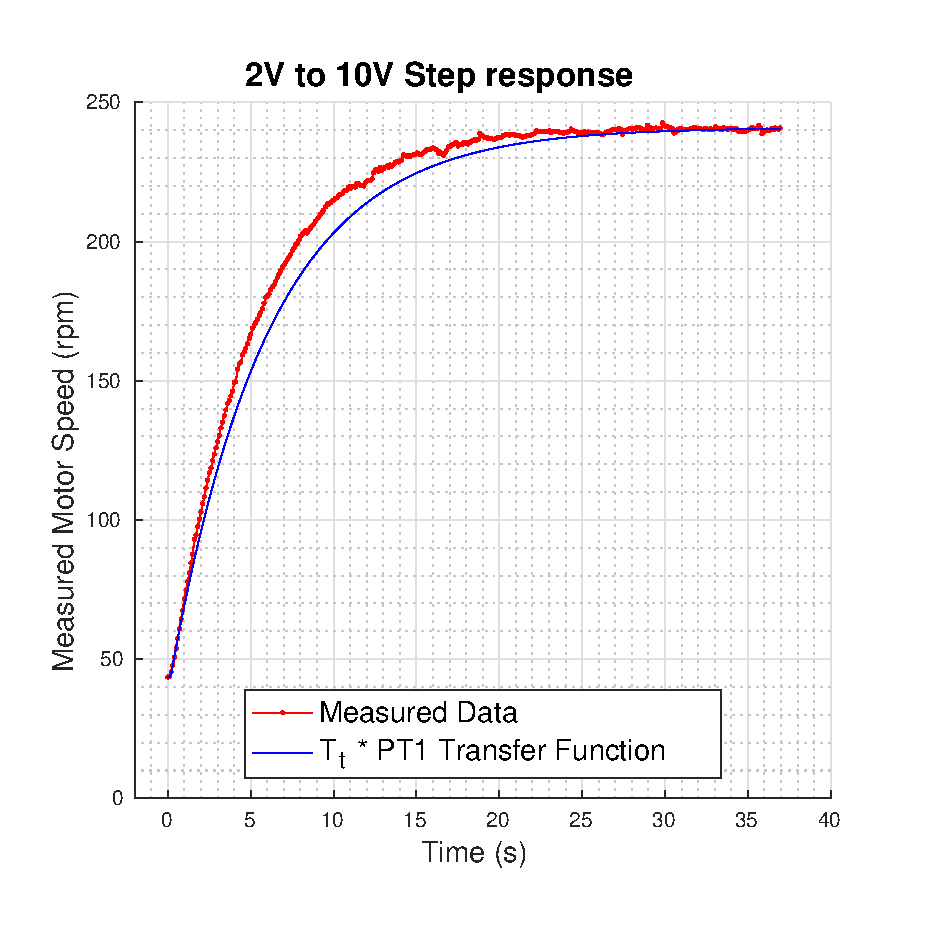
\includegraphics[width=\linewidth]{images/Tt_PT1}
    \caption{XXX}
\end{figure}

\begin{figure}
    \centering
    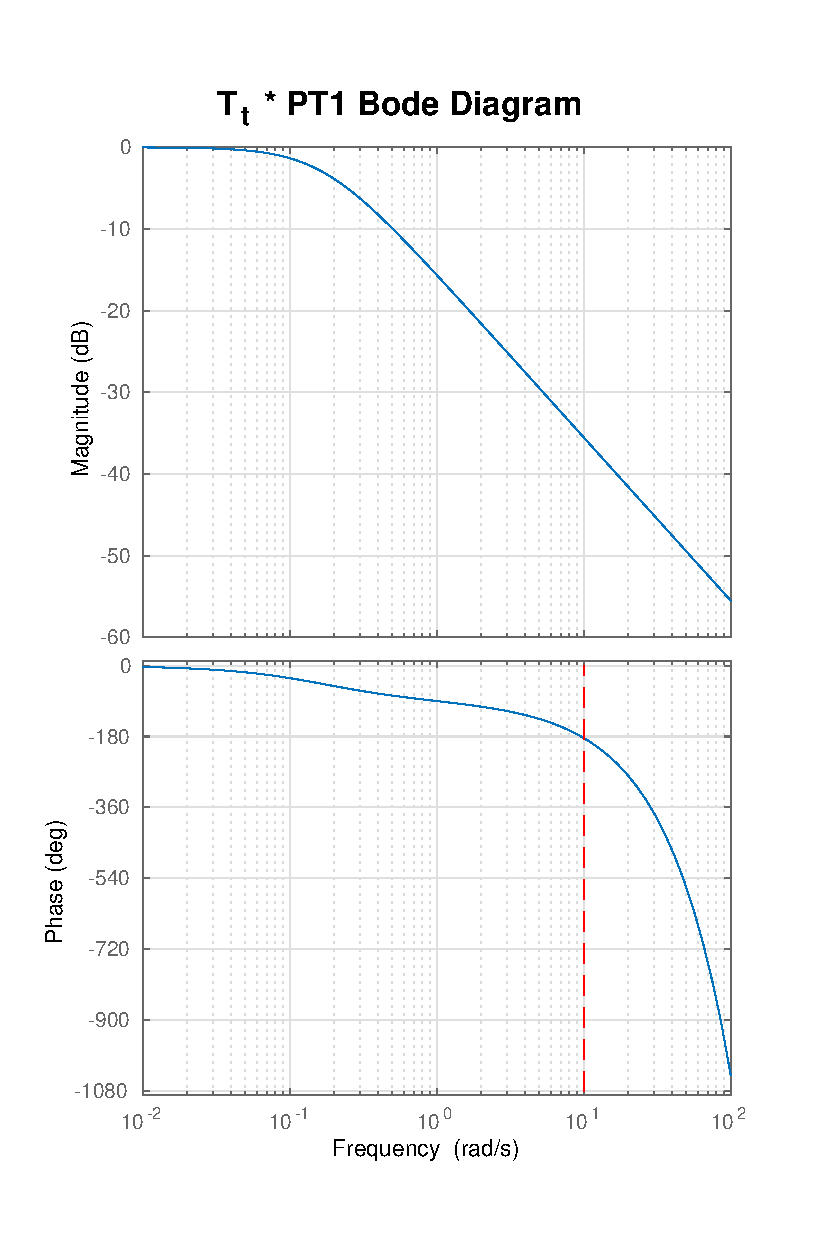
\includegraphics[width=\linewidth]{images/Tt_PT1_bode}
    \caption{XXX}
\end{figure}

\subsection{Simulation with simulink}
A simulation were done in simulink to compare the tracking behavior between simulation and experiment.
First we determine the parameter of the controller with the simulation in the picture 1.
The best value for the $PT_{1}$ we determine were $5.947$
so our $PT_{1}$ element is from the form:
\begin{equation}
G(s) = \frac{1}{5.947s+1}
\end{equation}